%%%%%%%%%%%%%%%%%%%%%%%%%%%%%%%%%%%%%%%%%
% Friggeri Resume/CV
% XeLaTeX Template
% Version 1.0 (5/5/13)
%
% This template has been downloaded from:
% http://www.LaTeXTemplates.com
%
% Original author:
% Adrien Friggeri (adrien@friggeri.net)
% https://github.com/afriggeri/CV
%
% License:
% CC BY-NC-SA 3.0 (http://creativecommons.org/licenses/by-nc-sa/3.0/)
%
% Important notes:
% This template needs to be compiled with XeLaTeX and the bibliography, if used,
% needs to be compiled with biber rather than bibtex.
%
%%%%%%%%%%%%%%%%%%%%%%%%%%%%%%%%%%%%%%%%%
\documentclass[a4paper]{friggeri-cv-white} % Add 'print' as an option into the square bracket to remove colors from this template for printing
\XeTeXinputencoding "latin1" % codage du document
%\addbibresource{bibliography.bib} % Specify the bibliography file to include publications
\bibliography{bibliography}
\usepackage{enumitem}
\usepackage{fancyhdr}
\usepackage{hyperref} 
\fancypagestyle{plain}{
    \fancyhf{} %Clear Everything.
    \fancyfoot[C]{} %Page Number
    \renewcommand{\headrulewidth}{0pt} %0pt for no rule, 2pt thicker etc...
    \renewcommand{\footrulewidth}{0pt}
    \fancyfoot[L]{}
    %\fancyfoot[R]{\color{gray}\thepage/\pageref{lastpage}}
    \fancyhead{}
    \fancyhead{}
}
\pagestyle{plain}

\begin{document}


%\let\cleardoublepage\clearpage
%\header{Rony}{Rozas}{Consultant en datamining} % Your name and current job title/field
\header{Data}{Scientist}{Rony Rozas}
%\header{Rony}{Rozas}{Ing�nieur R\&D} % Your name and current job title/field
%\header{Rony}{Rozas}{Ing�nieur M�thodes Maintenance}
%\header{Rony}{Rozas}{Ing�nieur en Optimisation} % Your name and current job title/field

%----------------------------------------------------------------------------------------
%	SIDEBAR SECTION
%----------------------------------------------------------------------------------------

\begin{aside} % In the aside, each new line forces a line break
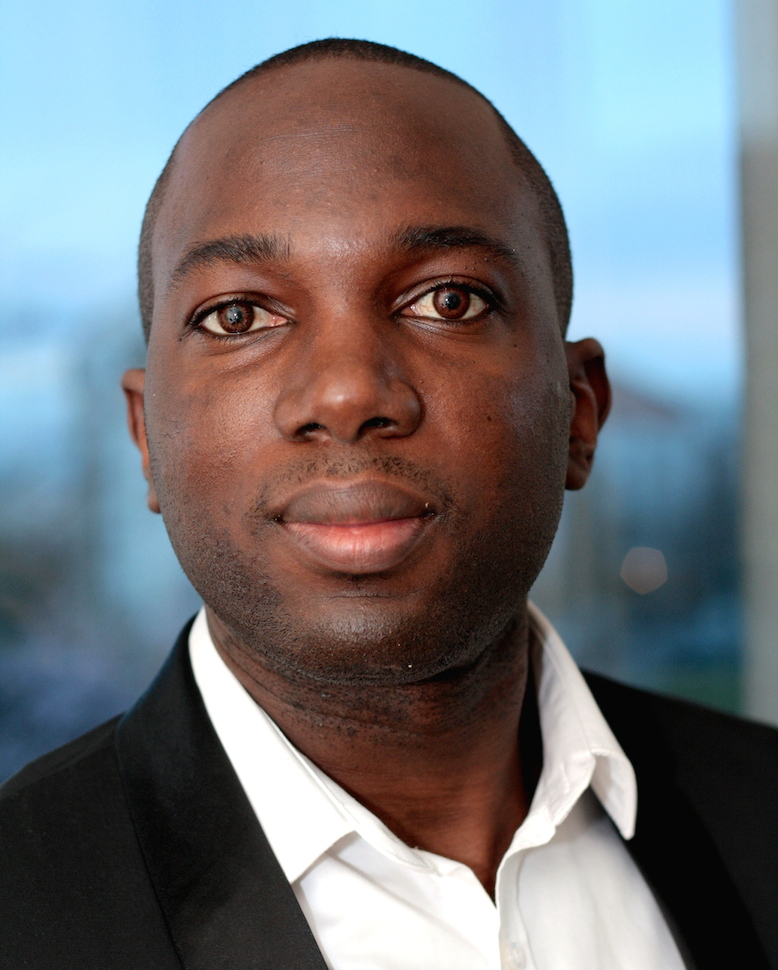
\includegraphics[width=0.17\paperwidth]{IMG_5630.JPG}
\section{Contact}
16 Rue de Bietighiem
94370 Sucy-en-Brie 
~
{\color{red}\mobilephonesymbol} +33 (0) 6 50 27 43 11
%{\color{red}\fixedphonesymbol} +33 (0) 1 81 66 86 92
{\color{red}\emailsymbol} \href{mailto:rozas.rony@gmail.com}{rozas.rony@gmail.com}
%\href{http://www.ronyrozas.com}{http://www.ronyrozas.com}
%\href{https://www.linkedin.com/in/rony-rozas-ab046659}{linkedin}
~
Fran\c{c}ais, 32 ans
%\section{Keywords}
%Machine Learning
%Big Data
%Optimisation
%Stochastics process
%Natural Language Processing
%~
%\section{Languages}
%\begin{entrylist}
%------------------------------------------------
%\entryinline{Fran�ais}{Langue maternelle}
French : Mother tongue
English : Professional %Lu, \'{e}crit, parl\'{e}
Spanish : Notions
%\entryinline{Anglais}{Lu, \'{e}crit, parl\'{e}}
%\entryinline{Espagnol}{Notions}
%\end{entrylist}
~
\section{References}
~
Patrick Marty 
Search Engine Manager
{\small \itshape FNAC }
\href{mailto:marty.patrick@gmail.com}{marty.patrick@gmail.com}
%+33 (0)6 72 29 35 07
~
St�phane Soulier 
S�nior DataScientist
{\small \itshape Pretty Simple}
\href{mailto:stephane@soolier.com}{stephane@soolier.com}
%+33 (0)6 24 64 79 67
~
Patrice Aknin
Scientific Director
{\small \itshape IRT SystemX}
\href{mailto:patrice.aknin@ifsttar.fr}{patrice.aknin@ifsttar.fr}
%+33 (0)1 57 23 62 92 
%~
%Laurent Bouillaut
%{\small \itshape IFSTTAR}
%Charg� de recherche
%+33 (0)1 81 66 87 16 
%~
%Nihal Pekergin - {\small \itshape UPEC}
%Enseignant / chercheur
%+33 (0)1 45 17 16 44
%~
\section{Interests}
Volley-ball, Roller-skates, Salsa, Kaggle, Datascience.net\vspace{\parsep}
\end{aside}

%----------------------------------------------------------------------------------------
%	WORK EXPERIENCE SECTION
%----------------------------------------------------------------------------------------

\section{Skills}

\subsection{Scientifics}
\begin{entrylist}
%------------------------------------------------
%\entryinline
%{M�thodes}
%{\emph{Big Data} : Hadoop, Hive, Pig \\[0.3em]
%\emph{Machine Learning} : Arbres de d�cision, K-Means, K-Nearest Neighbors, SVM, Gradient boosting model, Random Forest, Neural networks \\[0.3em]
%\emph{Statistiques} : R�gression lin�aire, Estimateurs, Tests d'hypoth�ses, ANOVA\\[0.3em]
%\emph{Optimisation} : Programmation dynamique, Programmation par contraintes, Programmation Lin�aireL, Combinatoire, Multicrit�re, M�taheuristique,   \\[0.3em]
%\emph{Processus stochastiques} : R\'{e}seaux Bay\'{e}siens, Cha\^{i}ne de Markov 
%%Data Mining, Planification, Machine Learning, Mod�lisation math�matique
%}

\entryinline{Machine Learning} {Decision trees, K-Nearest Neighbors, Gradient Boosting Machine, Neural networks, Random Forest, K-Means, Support Vector Machine}
\entryinline{Statistics} {Linear regression, Estimators, Statistical hypothesis testing, ANOVA }
\entryinline{Optimization} {Dynamic programming, Constraint programmming, Linear programming, Multi-objective optimization, Combinatorial optimization, Metaheuristics }

%\entryinline{Processus stochastiques}{R\'{e}seaux Bay\'{e}siens, Cha\^{i}ne de Markov } 
%Data Mining, Planification, Machine Learning, Mod�lisation math�matique

%------------------------------------------------
\end{entrylist}

\subsection{Computer Science}
\begin{entrylist}
%------------------------------------------------
\entryinline
{Languages}
{Python (Numpy, Scipy, Pandas, Scikit-learn) , R, Java, C++, C, Bash }
%------------------------------------------------
%\entryinline
%{Outils}
%{Matlab, Maple, Octave}
%------------------------------------------------
%\entryinline
%{Big Data}
%{Hadoop, MapReduce, Hive, Pig}
%%------------------------------------------------
%\entryinline{Search Engine}{SolR, Elasticsearch}
%%------------------------------------------------
\entryinline{Analytics}{Penthao, Tableau Software, Business Catalyst}
%\entryinline
%{Graphisme}
%{Adobe Creative Suite : Photoshop, Illustrator, InDesign, Flash}
%%------------------------------------------------
%\entryinline
%{SGBD}
%{MySQL, PosgreSQL  }
%------------------------------------------------
%\entryinline{Syst\`{e}mes}
%{Windows, Linux}
%------------------------------------------------
\end{entrylist}
\begin{entrylist2}
\entryinlineS
{Big Data}{Hadoop, Hive, Pig, Spark}
{Database}{MySQL, PosgreSQL  }
%------------------------------------------------
\entryinlineS
{Indexation engine}{SolR, Elasticsearch}
{Tools}{Matlab, Maple, Octave}
\end{entrylist2}

\subsection{Transversal}
\begin{entrylist}
\entryinline
{Intellectual}
{Analysis and synthesis capacity, Organization, Conceptualization, Ability to conduct an information and technology watch }
% autre : interdisciplinarit�, capacit� de prise de risques lors de d�cisions, maturit� et ma�trise �motionnelle et contr�le de soi, mode de r�flexion, aptitude � expliciter son cheminement et ses choix, interdisciplinarit�
\entryinline
{Social}
{Creation of competence networks, Communication, Good listening skills, pedagogy}
% autre : ouverture d'esprit et sens de l'humain, recherche et besoin de contacts sociaux, besoin de reconnaissance et d'encouragement, confiance envers les autres, 
%\entryinline
%{Organisationnelles}
%{}
%\entryinline
%{M�thodologique}
%{}
\end{entrylist}

\section{Experience}

\begin{entrylist}
%------------------------------------------------
\entry
{2015 - Now}
{DataScientist / Search Engine Engineer - {\normalfont \itshape \small LeGuide Group}}
{Paris, France}
{ Improve search results relevance using datamining and maching learning tools : 
\begin{itemize}
\item Using supervised and unsupervised classification methods applied to the categorization of millons products in thousands categories
\item Optimization of advertising and SEO campaigns
\item Analysis and rewriting user search queries 
\end{itemize}
}
%------------------------------------------------%------------------------------------------------
\entry
{2014 - 2015}
{Consultant DataScientist - {\normalfont \itshape \small Quantmetry}}
{Paris, France}
{Consulting with major players in the insurance, banking, complementary health and car rentals : 
\begin{itemize}
\item Predicting the palatability of a customer to take a loan.
\item Fraude detection in a mutual health insurance
\item Predicting the probability of a new transaction for a customer given his transaction history
\end{itemize}
}
%------------------------------------------------
\entry
{2010 - 2014}
{PhD candidate in Applied Mathematics - {\normalfont \itshape \small GRETTIA / IFSTTAR}}
{Marne-la-Vall\'{e}e, France}
{Projet whith  \textsc{Bombardier} : 
\begin{itemize}
\item Conception of a decision support tool to reduce the risk of downtime and ensure a high level of safety for train doors.
\item Establishment of a technical optimization of maintenance parameters. 
%\item D\'{e}veloppement d'une technique d'optimisation dynamique de param\`{e}tres de maintenance.
\item Probabilistic modeling of reliability.
% \`{a} partir de flux de  donn\'{e}es sur la fiabilit\'{e} de syst\`{e}mes multi-composants.
\end{itemize}
}
%------------------------------------------------
\entry
{2010 - 2014}
{Teacher - {\normalfont \itshape Universit\'{e} Paris-Est Cr\'{e}teil}}
{Cr\'{e}teil, France}
{Sofware engineering, algorithmic, object-oriented programming (Java), imperative programming (C)}
%------------------------------------------------
%\entry
%{2013 - 2014}
%{Attach\'{e} Temporaire d'Enseignement et de Recherche}
%{Cr\'{e}teil, France}
%{Universit\'{e} Paris Est Cr\'{e}teil \\
%Enseignement de modules de g\'{e}nie logiciel, de programmation orient\'{e}e objet et d'algorithmique.}
%%------------------------------------------------
%\entry
%{2010 - 2013}
%{Mission d'enseignement}
%{Cr\'{e}teil, France}
%{Universit\'{e} Paris Est Cr\'{e}teil \\
%Enseignement de modules d'algorithmique, de programmation orient\'{e}e objet en Java et de programmation imp\'{e}rative en C.}
%------------------------------------------------
%\entryL
%{2009 {\small (6 mois)}}
%{Ing�nieur en optimisation (stagiaire) - {\normalfont \itshape \small INRA / %IRIT}}
%{Toulouse, France}
%{\begin{itemize}
%\item D\'{e}veloppement d'algorithmes d'optimisation de pr\'{e}f\'{e}rences multicrit\`{e}res.  
%\item Utilisation du formalisme des probl\`{e}mes de satisfactions de contraintes pond\'{e}r\'{e}es ( {\small VCSP} )
%\end{itemize}}
%------------------------------------------------
%\entry
%{2009 {\small (4 mois)}}
%{Concepteur/D\'{e}veloppeur - {\normalfont \itshape PizzaCap}}
%{Toulouse, France}
%{Conception d'une application client/serveur de prise de commandes (Windev).}
%%{Conception et r\'{e}alisation d'une application client/serveur de prise de commande (Windev).}
%\end{entrylist}
%\begin{entrylist}
%------------------------------------------------
%\entryF
%{2008 {\small (5 mois)}}
%{Tuteur - {\normalfont \itshape Universit\'e{} des Antilles et de la Guyane}}
%{Martinique, France}
%Tutorat de lyc\'{e}en en math\'{e}matiques et physique}
%------------------------------------------------
%\entry
%{Juillet 2006}
%{Emploi saisonnier}
%{Guadeloupe, France}
%{A\'{e}roport P\^{o}le Cara\"{i}bes}
%Accueil et information des voyageurs}
%------------------------------------------------
\end{entrylist}





%----------------------------------------------------------------------------------------
%	EDUCATION SECTION
%----------------------------------------------------------------------------------------

\section{Education}

\begin{entrylist}
%------------------------------------------------
\entryF
{2014}
{PhD {\normalfont -- Computer Science and Applied Mathematics}}
{Universit\'e{} Paris-Est}

%------------------------------------------------
\entry
{2009}
{Master {\normalfont -- Computer Science and Telecom}}
{Universit\'e{} Paul Sabatier}
{speciality : Artificial intelligence}
%------------------------------------------------
%\entry
%{2007}
%{Licence {\normalfont -- STS (Sciences Technologies Sant\'e{})} }
%{Universit\'e{} des Antilles et de la Guyane}
%{sp\'{e}cialit\'{e} :  Informatique}
%------------------------------------------------
%\entry
%{2006}
%%{Dipl\^{o}me d'\'{e}tudes universitaires g\'{e}n\'{e}rale {\normalfont -- MIAS (Math\'e{}matiques Informatiques et Applications aux Sciences)}}
%{Dipl�me d'�tudes universitaires g�n�rale {\normalfont -- MIAS (Math\'e{}matiques Informatiques et Applications aux Sciences)}}
%{Universit\'e{} des Antilles et de la Guyane}
%{sp\'{e}cialit\'{e} :  Informatique}
%------------------------------------------------
%\entryF
%{2004}
%{Classe pr\'{e}paratoire aux grandes \'{e}coles {\normalfont-- MPSI (Math\'e{}matiques Physique et Sciences de l'ing\'e{}nieur)}}
%{Lyc\'e{}e G\'e{}n\'e{}ral et Technologique de Baimbridge}

\end{entrylist}

\vspace{-20pt}
%----------------------------------------------------------------------------------------
%	COMMUNICATION SKILLS SECTION
%----------------------------------------------------------------------------------------
%
%\section{communication skills}
%
%\begin{entrylist}
%%------------------------------------------------
%\entry
%{2011}
%{Oral Presentation}
%{California Business Conference}
%{Presented the research I conducted for my Masters of Commerce degree.}
%%------------------------------------------------
%\entry
%{2010}
%{Poster}
%{Annual Business Conference, Oregon}
%{As part of the course work for BUS320, I created a poster analyzing several local businesses and presented this at a conference.}
%%------------------------------------------------
%\end{entrylist}

%----------------------------------------------------------------------------------------
%	INTERESTS SECTION
%----------------------------------------------------------------------------------------

%\section{Centres d'int\'{e}r\^{e}t}
%\begin{entrylist}
%\entryinline{Loisirs}{Volley-ball, roller, salsa, Kaggle }
%\entryinline{Associatif}{Responsable de l'association de danse latine de l'Universit\'{e} de Marne-la-Vall\'{e}e}
%\end{entrylist}

%----------------------------------------------------------------------------------------
%	PUBLICATIONS SECTION
%----------------------------------------------------------------------------------------

%\section{Publications}

%\printbibsection{article}{article in peer-reviewed journal} % Print all articles from the bibliography
%\nocite{*}
%\printbibliography[ type=article, title={Articles}, heading=subbibliography]
%\printbibsection{book}{books} % Print all books from the bibliography

%\begin{refsection} % This is a custom heading for those references marked as "inproceedings" but not containing "keyword=france"
%\nocite{*}
%\printbibliography[ type=inproceedings, title={international peer-reviewed conferences/proceedings}, notkeyword={france}, heading=subbibliography]
%\end{refsection}

%\begin{refsection} % This is a custom heading for those references marked as "inproceedings" and containing "keyword=france"

%\printbibliography[heading=subbibliography]
%\end{refsection}

%\printbibsection{misc}{other publications} % Print all miscellaneous entries from the bibliography

%\printbibsection{report}{research reports} % Print all research reports from the bibliography
 	
%----------------------------------------------------------------------------------------

%\section{R�f�rences}
%\begin{tabular}{p{3 cm}p{7.3cm}p{3.5cm}}
%Patrice Aknin & Directeur scientifique � la {\small SNCF} & +33 (0)1 57 23 62 92 \vspace{\parsep}\\%+33 (0)6 07 44 96 13 
%Laurent Bouillaut & Charg� de recherche � l'{\small IFSTTAR}& +33 (0)1 81 66 87 16\vspace{\parsep}\\
%Nihal Perkergin & Enseignant / chercheur � l'{\small UPEC} &+33 (0)1 45 17 16 44\vspace{\parsep}\\
%\end{tabular} 
\label{lastpage}

\end{document}
